\begin{filecontents*}[overwrite]{example-references.bib}
@book{knuth1984texbook,
  author    = {Donald E. Knuth},
  title     = {The TeXbook},
  year      = {1984},
  publisher = {Addison-Wesley}
}

@article{lamport1986latex,
  author  = {Leslie Lamport},
  title   = {Document Preparation Systems},
  journal = {Software: Practice and Experience},
  year    = {1986},
  volume  = {16},
  number  = {6},
  pages   = {531--542}
}

@inproceedings{sterling2025workflows,
  author    = {Ada Sterling and Benoit Sample},
  title     = {Reproducible Workflows for Small Simulation Teams},
  booktitle = {Proceedings of the Example Research Software Workshop},
  year      = {2025},
  pages     = {12--21}
}
\end{filecontents*}

\providecommand{\oritoneexamplemode}{white}
\documentclass[english,\oritoneexamplemode,bibtex]{oritone-thesis}

\title{A Complete Thesis Example for Scientific Software Workflows}
\author{Ada Sterling}
\date{\today}

\universityName{Example University}
\universityLogo{example-image-a}
\universityLogoWidth{7cm}
\studyProgram{Computational Engineering}
\desiredDegree{Master of Science}
\firstExaminer{Prof. A. Example}{Computational Methods}
\secondExaminer{Prof. B. Sample}{Software Systems}
\thesisSubject{Thesis class demonstration}
\thesisKeywords{LaTeX, thesis, document class, scientific software}
\thesisBibliographyResource{example-references}

\begin{document}
\frontmatter
\maketitle

\abstractChapter
This example demonstrates the thesis class with realistic front matter,
chapter headings, equations, figures, subfigures, tables, listings, plots,
cross-references, bibliography output, and a declaration page. The topic is a
small scientific software workflow because it naturally exercises mathematical
notation, implementation detail, and experimental reporting.

The text is intentionally longer than a minimal example. Filled pages make it
easier to evaluate margins, running heads, page numbers, caption spacing,
chapter starts, and the balance between the Oritone color layer and standard
black-on-white thesis pages.

\chapter*{Acknowledgements}
The author thanks the Example Laboratory for discussions about reproducible
computing, the thesis supervisors for careful review, and the package
maintainers who keep the LaTeX ecosystem reliable.

\tableofcontents
\listoffigures
\listoftables

\mainmatter
\chapter{Introduction}
\label{ch:introduction}

\section{Motivation}
\label{sec:motivation}

Scientific software projects often begin as small experiments. A researcher
tests a model, saves a few plots, and shares a notebook with a collaborator.
When the same workflow becomes part of a thesis, the requirements change:
inputs need names, artifacts need provenance, figures need stable generation,
and numerical claims need enough context to be checked later.

This thesis example treats the document class as part of that workflow. The
title page stores institutional metadata, the front matter contains the usual
abstract and lists, and the main matter demonstrates the notation and reporting
surfaces that appear in a compact computational thesis. The class also provides
short helpers such as \verb|\bs| for bold symbols, \verb|\intd| for integration
measures, \verb|\Assembly| for assembly notation, and \verb|\linktt| for
monospaced links such as \linktt{https://example.com/oritone}.

\section{Contributions}
\label{sec:contributions}

The example is structured around four contributions. First, it introduces a
small model problem in \Cref{ch:model}. Second, it shows how tables and
listings sit inside a chapter with standard thesis spacing. Third, it uses
PGFPlots and subfigures in \Cref{ch:results}. Fourth, it closes with a
bibliography and declaration page so that the generated PDF resembles a complete
thesis rather than an isolated chapter.

\begin{enumerate}
  \item A reproducible text source that exercises class metadata and front
    matter.
  \item A compact mathematical model with equations and assembly notation.
  \item Tables, listings, and plots using the shared color and font layer.
  \item Back matter that demonstrates bibliography and declaration commands.
\end{enumerate}

\begin{oritonenote}[Document Role]
The thesis class exposes the same semantic callout surface as the manuscript
class, but keeps the surrounding page geometry, headings, and front matter
appropriate for a long-form document.
\end{oritonenote}

\section{Related Work}
\label{sec:related-work}

The example bibliography is intentionally small. It cites a classic typesetting
reference \cite{knuth1984texbook} and a document preparation reference
\cite{lamport1986latex}. It also cites a fictional workflow paper
\cite{sterling2025workflows}. The bibliography mechanism remains configurable:
the document can use BibTeX, or the class option can switch to BibLaTeX when a
project needs that toolchain.

\chapter{Model and Discretization}
\label{ch:model}

\section{Weak Form}
\label{sec:weak-form}

Let \(\Omega\subset\mathbb{R}^d\) be a bounded domain and let
\(\bs{u}:\Omega\to\mathbb{R}^d\) denote a displacement field. A compact weak
form for a linear elastic model is: find \(\bs{u}\in V\) such that
\begin{equation}
  \int_\Omega
    \bs{\varepsilon}(\delta\bs{u}) : \bs{C} :
    \bs{\varepsilon}(\bs{u})
  \intd{\Omega}
  =
  \int_\Omega
    \delta\bs{u}\cdot\bs{p}
  \intd{\Omega}
  \qquad \forall\delta\bs{u}\in V .
  \label{eq:weak-form}
\end{equation}
The notation in \Cref{eq:weak-form} is deliberately conventional. It is useful
for exercising bold symbols, display math, equation labels, and the slightly
expanded line spacing of the thesis class.

\subsection{Element Assembly}
\label{sec:assembly}

On a mesh \(\mathcal{T}_h\), the element contributions are accumulated with
assembly notation,
\begin{equation}
  \bs{K}
  =
  \Assembly_{T\in\mathcal{T}_h}
  \int_T
    \bs{B}_T^\mathsf{T}\bs{C}\bs{B}_T
  \intd{x},
  \qquad
  \bs{f}
  =
  \Assembly_{T\in\mathcal{T}_h}
  \int_T
    \bs{N}_T^\mathsf{T}\bs{p}
  \intd{x}.
  \label{eq:assembly}
\end{equation}
The helper \(\Assembly\) is available for this common notation. A draft note can
also be marked inline: \todo{verify boundary-condition wording before
submission}. That command remains visually distinct without changing the page
structure.

\begin{oritonewarning}[Draft Checkpoint]
Inline todo text is useful for small reminders. A warning callout is better when
an unresolved issue affects a full derivation, experiment, or chapter section.
\end{oritonewarning}

\begin{table}[tbp]
  \centering
  \caption{Discretization levels used in the example experiments.}
  \label{tab:levels}
  \begin{tabular}{rrrr}
    \toprule
    Level & Elements & Unknowns & Quadrature points \\
    \midrule
    1 & 64 & 162 & 256 \\
    2 & 256 & 578 & 1024 \\
    3 & 1024 & 2178 & 4096 \\
    4 & 4096 & 8450 & 16384 \\
    \bottomrule
  \end{tabular}
\end{table}

\section{Implementation Sketch}
\label{sec:implementation-sketch}

Listings are useful in a thesis when code fragments are short enough to support
the explanation. The class uses the same framed listing component as the other
Oritone document classes, while the listing itself selects Julia highlighting.

\begin{lstlisting}[language=Julia, caption={Residual accumulation for a toy element loop.}, label={lst:solver}]
function residual(cells, state)
  total = 0.0
  for cell in cells
    element = assemble_cell(cell, state)
    total += norm(element.force - element.stiffness * element.value)
  end
  return total
end
\end{lstlisting}

\Cref{lst:solver} is intentionally small. Longer production code should usually
live in a repository, while the thesis includes only the fragments needed to
support the argument.

\chapter{Results}
\label{ch:results}

\section{Convergence}
\label{sec:convergence}

The convergence data in \Cref{tab:convergence} are generated values for
demonstration. They give the page a realistic mix of text, numbers, captions,
and mathematical notation. The plot in \Cref{fig:error-plot} uses the shared
PGFPlots cycle list configured by the class.

\begin{table}[tbp]
  \centering
  \caption{Example convergence data for two solver variants.}
  \label{tab:convergence}
  \begin{tabular}{rrrr}
    \toprule
    Level & Standard error & Stabilized error & Time (s) \\
    \midrule
    1 & \(1.83\times10^{-1}\) & \(2.40\times10^{-1}\) & 0.8 \\
    2 & \(4.61\times10^{-2}\) & \(7.20\times10^{-2}\) & 2.7 \\
    3 & \(1.16\times10^{-2}\) & \(2.20\times10^{-2}\) & 9.4 \\
    4 & \(2.90\times10^{-3}\) & \(6.90\times10^{-3}\) & 34.1 \\
    \bottomrule
  \end{tabular}
\end{table}

\begin{figure}[tbp]
  \centering
  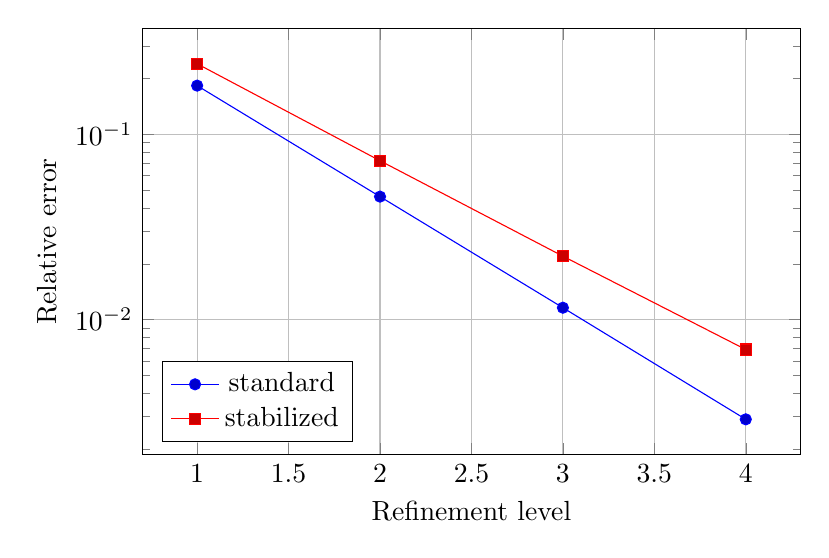
\begin{tikzpicture}
    \begin{axis}[
      width=0.82\textwidth,
      height=7cm,
      xlabel={Refinement level},
      ylabel={Relative error},
      ymode=log,
      grid=major,
      legend pos=south west
    ]
      \addplot coordinates {(1,1.83e-1) (2,4.61e-2) (3,1.16e-2) (4,2.90e-3)};
      \addlegendentry{standard}
      \addplot coordinates {(1,2.40e-1) (2,7.20e-2) (3,2.20e-2) (4,6.90e-3)};
      \addlegendentry{stabilized}
    \end{axis}
  \end{tikzpicture}
  \caption{A PGFPlots figure using the shared cycle list.}
  \label{fig:error-plot}
\end{figure}

\section{Visual Diagnostics}
\label{sec:visual-diagnostics}

Thesis chapters frequently mix generated figures with explanatory text. The
subfigures in \Cref{fig:diagnostics} use placeholder images from the standard
LaTeX distribution, but the layout mirrors a typical pair of mesh or residual
diagnostics.

\begin{figure}[tbp]
  \centering
  \begin{subfigure}{0.45\textwidth}
    \centering
    \includegraphics[width=\linewidth]{example-image-b}
    \caption{Reference configuration.}
    \label{fig:diagnostic-reference}
  \end{subfigure}
  \hfill
  \begin{subfigure}{0.45\textwidth}
    \centering
    \includegraphics[width=\linewidth]{example-image-c}
    \caption{Perturbed configuration.}
    \label{fig:diagnostic-perturbed}
  \end{subfigure}
  \caption{Subfigures with caption styling supplied by the thesis class.}
  \label{fig:diagnostics}
\end{figure}

The diagnostics show how captions, subcaptions, and body text share the same
font layer. A filled page is the best way to see whether those defaults are too
large, too decorative, or too cramped. The class keeps the visual emphasis on
chapter structure and technical content.

\chapter{Conclusion}
\label{ch:conclusion}

The unified thesis class supplies the repeated structure needed for a complete
computational thesis: title metadata, front matter, compact chapter headings,
running heads, tables, captions, listings, plots, bibliography support, helper
math commands, and a declaration page. The example also demonstrates that the
white mode remains compatible with standard thesis expectations while still
using Oritone semantic colors for links, listings, rules, and plots.

Future projects can change fonts or color modes in the shared package layer
without rewriting individual thesis sources. That separation is the main design
goal: document authors write thesis content, while the class owns the common
presentation decisions.

\backmatter
\printThesisBibliography
\declarationOfAcademicIntegrity

\end{document}
